One of the strengths of \matlab is in its large library, which doesn't
only provide access to a large number of matrix computation functions,
but packages for other scientific fields. Even relatively simple
programs tend to use a fair number of library functions.  Many library
functions are actually implemented in \matlab code. Thus, to provide
their functionality, the callgraph construction needs to include any
\matlab function on the \matlab path, if it is available. In this way we can
provide access to a large number of library functions as long as we can
support the language features they use.  However, hundreds of \matlab
functions are actually implemented in native
code. We call these functions builtins or builtin functions.

Every \matlab operator (such as $+$, $*$) is also a builtin function;
the operations are merely syntactic sugar for calling the functions
that represent the operations (like {\tt plus} for {\tt +}, {\tt
mtimes} for {\tt *}).

For an accurate static analysis of \matlab
programs one requires an accurate model of the builtins.  In this
section we describe how we have modelled the builtins and how we
integrate the analysis into the static interprocedural analysis
framework.

\section{Learning about Builtins}

As a first step to build a framework of builtin functions, we need to
identify builtins, and need to find out about their behavior,
especially with respect to mclasses.

\subsection{Identifying Builtins}
\label{sec:idBuiltins}

To make the task of building a framework for builtins manageable, we
wanted to identify the most commonly used builtin functions and organize
those into a framework.   Other builtins can be added incrementally, but
this initial set was useful to find a good structure.

To identify commonly used builtins we used the \mcbench
framework\cite{SoroushThesis} to find all references to functions that
occur in a large corpus of over three thousand \matlab
programs.\footnote{This is the same set of projects that are used
in \cite{KindAnalysis}.  The benchmarks come from a wide variety of
application areas including Computational Physics, Statistics,
Computational Biology, Geometry, Linear Algebra, Signal Processing and
Image Processing.} We recorded the frequency of use for every function
and then, using the \matlab function {\tt exist}, which returns whether
a name is a variable, user-defined function or builtin, we identified
which of these functions is a builtin.  This provided us with
a list of builtin functions used in real \matlab programs, with their
associated frequency of use.  The complete list can be found
in \appendixref{chap:builtinList}.

We selected approximately three hundred of the most frequent
functions, excluding dynamic functions like {\tt eval} and 
graphical user interface functions as our
initial set of builtin functions. We also included all the functions
that correspond to \matlab operators, as well as some functions
that are closely related to functions in the list.




\subsection{Finding Builtin Behaviors}

In order to build a call graph it is very important to be able to
approximate the behavior of builtins.   More precisely,  given the
mclass of the input arguments,  one needs to know a safe approximation
of the mclass of the output arguments.   This behavior is actually
quite complex, and since the behavior of \matlab7 is the defacto
specification of the behavior we decided to take a programmatic
approach to determining the the behaviors.  

We developed a set of scripts that generate random \matlab values of all
combinations of builtin mclasses, and called selected builtins using these
arguments. If different random values of the same mclass result in
consistent resulting mclasses over many trials, 
the scripts record the associated mclass
propagation for builtins in a table, and collect functions with the
same mclass propagation tables together.   Examples of three 
such tables are given in \figref{Fig:BinOps}.
The complete list of result tables can be found in \appendixref{chap:allTables}


\begin{figure}[htbp]

%\fullreport{
 \begin{small}
 \renewcommand{\tabcolsep}{1.5pt}
%}

\begin{tabular}{c}
\begin{tabular}{cc}

\begin{tabular}{c}
%\fullreport{
  \begin{minipage}{3.0in}
%}
%\shortpaper{
%  \begin{minipage}{2.3in}
%}

\begin{tabular}{|l||l|l|l|l|l|l|l|l|} \hline
           &   {\tt i8} &  {\tt i16} &  {\tt i32} &   {\tt i64} &  {\tt f32} & {\tt f64}  & {\tt  c}   &  {\tt b}    \\ \hline \hline
 {\tt i8}  &  {\tt i8}  &   -        &   -        &   -         &    -       & {\tt i8}   & {\tt i8}   &  -          \\ \hline
 {\tt i16} &  -         &   {\tt i16} &   -       &   -         &    -       & {\tt i16}  & {\tt i16}  &  -          \\ \hline
 {\tt i32} &  -         &   -         & {\tt i32} &   -         &    -       & {\tt i32}  & {\tt i32}  &  -          \\ \hline
 {\tt i64} &  -         &   -         &   -       &   {\tt i64} &   -        & {\tt i64}  & {\tt i64}  &  -          \\ \hline
 {\tt f32} &  -         &   -         &   -       &   -         & {\tt f32}  & {\tt f32}  & {\tt f32}  & {\tt f32}   \\ \hline
 {\tt f64} &  {\tt i8}  &  {\tt i16}  & {\tt i32} &  {\tt i64}  & {\tt f32}  & {\tt f64}  & {\tt f64}  & {\tt f64}   \\ \hline
 {\tt c  }  & {\tt i8}  &  {\tt i16}  & {\tt i32} &  {\tt i64}  & {\tt f32}  & {\tt f64}  & {\tt f64}  & {\tt f64}   \\ \hline
 {\tt b  }  &  -        &   -         &   -       &   -         & {\tt f32}  & {\tt f64}  & {\tt f64}  & {\tt f64}   \\ \hline
\end{tabular}
\end{minipage}
\\
(a) {\tt plus}, {\tt minus}, {\tt mtimes}, {\tt times}, {\tt kron}
\end{tabular}


&

\begin{tabular}{c}
%\fullreport{
  \begin{minipage}{3.0in}
%}
%\shortpaper{
%  \begin{minipage}{2.3in}
%}

\begin{tabular}{|l||l|l|l|l|l|l|l|l|}
 \hline
           &   {\tt i8} &  {\tt i16}  &  {\tt i32} &  {\tt i64} &  {\tt f32} & {\tt  f64} & {\tt  c}   &  {\tt b}    \\ \hline \hline
 {\tt i8}  &   {\tt i8} &    -        &    -       &   -        &    -       &  -         & {\tt i8}   &  -          \\ \hline
 {\tt i16} &   -        &  {\tt i16}  &   -        &   -        &   -        &  -         & {\tt i16}  &  -          \\ \hline
 {\tt i32} &   -        &    -        &  {\tt i32} &   -        &   -        &  -         & {\tt i32}  &  -          \\ \hline
 {\tt i64} &   -        &   -         &   -        &  {\tt i64} &   -        &  -         & {\tt i64}  &  -          \\ \hline
 {\tt f32} &  -         &   -         &   -        &   -        & {\tt f32}  & -          & {\tt f32}  & {\tt f32}   \\ \hline
 {\tt f64} &  {\tt i8}  & {\tt i16}   & {\tt i32}  & {\tt i64}  & {\tt f32}  & {\tt f64}  & {\tt f64}  & {\tt f64}   \\ \hline
 {\tt c  } &  {\tt i8}  & {\tt i16}   & {\tt i32}  & {\tt i64}  & {\tt f32}  & {\tt f64}  & {\tt f64}  & {\tt f64}   \\ \hline
 {\tt b  } &  -         &   -         &   -        &   -        & {\tt f32}  & {\tt f64}  & {\tt f64}  & -           \\ \hline
\end{tabular}
\end{minipage}
\\
(b) {\tt mpower}, {\tt power}
\end{tabular}

\end{tabular}

\\ \\

\begin{tabular}{c}
%\fullreport{
  \begin{minipage}{3.0in}
%}
%\shortpaper{
%  \begin{minipage}{2.3in}
%}

\begin{tabular}{|l||l|l|l|l|l|l|l|l|} \hline
           &   {\tt i8} &  {\tt i16} &  {\tt i32} & {\tt i64} &  {\tt f32} & {\tt  f64}  & {\tt  c}  &  {\tt b}    \\ \hline \hline
 {\tt i8}  &   {\tt i8} &    -       &   -        &   -       &   -        & {\tt i8}    & {\tt i8}  &  -          \\ \hline
 {\tt i16} &    -       &  {\tt i16} &   -        &   -       &   -        & {\tt i16}   & {\tt i16} &  -          \\ \hline
 {\tt i32} &    -       &    -       &  {\tt i32} &   -       &   -        & {\tt i32}   & {\tt i32} &  -          \\ \hline
 {\tt i64} &    -       &   -        &   -        & {\tt i64} &   -        & {\tt i64}   & {\tt i64} &  -          \\ \hline
 {\tt f32} &  -         &   -        &   -        &   -       & {\tt f32}  & {\tt f32}   & {\tt f32} & {\tt f32}   \\ \hline
 {\tt f64} &  {\tt i8}  & {\tt i16}  & {\tt i32}  & {\tt i64} & {\tt f32}  & {\tt f64}   & {\tt f64} &{\tt f64}    \\ \hline
 {\tt c  } &  {\tt i8}  & {\tt i16}  & {\tt i32}  & {\tt i64} & {\tt f32}  & {\tt f64}   & {\tt f64} &{\tt f64}    \\ \hline
{\tt b  }  &   -        &   -        &   -        &   -       & {\tt f32}  & {\tt f64}   & {\tt f64} & -           \\ \hline
\end{tabular}
\end{minipage}
\\
(c) {\tt mldivide}, {\tt mrdivide}, {\tt ldivide}, {\tt rdivide}, {\tt mod}, {\tt rem}, {\tt mod}
\end{tabular}

\end{tabular}

%\fullreport{
\end{small}
%}


\caption[Example mclass results for groups of builtin binary operators]
{Example mclass results for groups of builtin binary operators.  Rows
correspond to the mclass of the left operand, columns correspond to
the mclass of the right operand, and the table entries give the mclass
of the result. The labels {\tt i8} through {\tt i64} represent the
mclasses {\tt int8} through {\tt int64}, {\tt f32} is {\tt single},
{\tt f64} is {\tt double}, {\tt c} is {\tt char}, and {\tt b} is {\tt
logical}.  Entries of the form ``-" indicate that this combination is
not allowed and will result in a runtime error.

To save space we have not included the complete generated table,
we have left out the columns and rows for
unsigned integer mclasses and for handles.}
\label{Fig:BinOps}
\end{figure}

As compared with type rules in other languages,  these results may seem
a bit strange.   For example, the ``-" entry for
{\tt plus(int16,int32)} in \figref{Fig:BinOps}(a) shows that it is
an error to add an {\tt int16} to and {\tt int32}.  However adding an {\tt int64} to a
{\tt double} is allowed and results in an {\tt int64}.   Also, note that although
the three tables in \figref{Fig:BinOps} are similar, they are not
identical.  For example, in \figref{Fig:BinOps}(a),  multiplying a
{\tt logical} with a {\tt logical} results in a {\tt double},  but using the power
operator with two {\tt logical} arguments throws an error.  Finally, note that the tables
are not always symmetrical.   In particular, the \texttt{f64} column and
row in \figref{Fig:BinOps}(b) are not the same.

The reader may have noticed how the superior/inferior m-class
relationships as shown in figure \figref{Fig:Superior} seem to resemble
the implicit type conversion rules for \matlab builtin functions. For
example, when adding an integer and a double, the result will be double.
However, it is not sufficient to model the implicit \matlab class
conversion semantics by just using class-specialized functions and their
relationships.  Many \matlab builtins perform explicit checks on the
actual runtime types and shapes of the arguments and perform different
computations or raise errors based on those checks. 

Through the collection of a large number of tables 
we found that many builtins have similar high-level behavior. We
found that some functions work on any matrix, some work on numeric data,
some only work on floats, and some work on arbitrary builtin values,
including cell arrays or function handles.

\section{Specifying Builtins}

To capture the regularities in the builtin behavior, we arranged all of
the builtins in a hierarchy - a part of the hierarchy is given in
\figref{Fig:Builtin}.   Leaves of the hierarchy correspond to actual
builtins and internal nodes correspond to abstract builtins or a grouping of builtins which share some
 similar behavior.


\begin{figure}[htbp]
\begin{center}
\includegraphics[width=5in]{Figures/floatTree.eps}
\caption[Subtree of the builtin tree, showing defined float functions]{
  Subtree of the builtin tree, showing all defined floating point
  builtins of \matlab. All internal nodes are abstract builtins, the 
  names inside the boxes refer to actual functions.  
  The full tree showing all defined builtins is available at \url{http://www.sable.mcgill.ca/mclab/tamer.html}.}
\label{Fig:Builtin}
\end{center}
\end{figure}




\begin{figure}[htbp]
\lstinputlisting[language=python,nolol=true]{code/spec}
\caption[Excerpt of builtin specification]{Excerpt of the builtin specification, showing definitions
 for some of the floating point functions shown in \figref{Fig:Builtin}.
 The lines starting with a \#-symbol are comments.}
\label{Fig:Spec}
\end{figure}



To specify the builtins and their tree-structure, we developed a
simple domain-specific language.  A builtin is specified by values on
one line.  Values on every line are separated by semicolons.  To
specify a builtin, the first value has to be the name of the builtin.

If the builtin is abstract, i.e. it refers to a group of builtins, 
the parent group has to be specified as a second value.
If no parent is specified, the specified builtin is a concrete
builtin, belonging to the group of the most recently specified
abstract builtin. This leads to a very compact representation, 
a snippet of which is shown in \figref{Fig:Spec}.


Values after the second are used to specify properties or
attributes of builtins. Attributes can be specified for abstract
builtins, meaning that all children nodes will have that attribute.
This motivates structuring all builtins in a tree - if similar builtin
functions have the same attributes, then we may only have to specify
properties once.

The builtin framework takes a specification like shown
in \figref{Fig:Spec} as input, and generates a set of Java classes,
one for each builtin function, whose inheritance relationship reflects
the specified tree. For an abstract builtin, the generated Java class
is abstract as well. The builtin framework (the code that 
generates Java files from the builtin specification) is written in Python.


\subsection{Builtin Visitor Class}

Besides the builtin classes, the builtin framework also generates a
visitor class in Java.  It allows adding methods to builtins and
thus to define flow equations for them using the visitor pattern - a pattern
that is already extensively used in the \mcsaf analysis
framework\cite{JesseThesis}. In fact, flow analyses themselves are
written using the visitor pattern.
\vspace{.5cm}

\begin{figure}
\hspace{-.3cm}
\begin{minipage}{1.018\textwidth}
\lstinputlisting[language=Java,nolol=true]{code/visitor}
\caption[Excerpt of the generated builtin visitor class]{
Excerpt of the visitor class {\tt BuiltinVisitor} that is generated by the builtin framework using
the specification shown in \figref{Fig:Spec}. The comments are copied
from the specification file by the builtin framework.}
\label{Fig:visitor}
\end{minipage}
\end{figure}

The generated visitor class (see \figref{Fig:visitor}) can be used to
make flow analyses implement flow equations for all builtins.  In
order to do so, \rednote{one} has to derive from the visitor class and fill in the
class variables used as argument and return values for the case
methods. Overriding case methods allows specifying desired flow equations for
the corresponding builtin.

Note that the default case for every builtin is to call the parent
case - this means that to specify behavior for similar builtins, one
only needs to specify the abstract behavior of a group, and the flow
analysis framework will automatically apply the correct (most
specialized) behavior for a specific builtin.  This further motivates
the structuring of builtin functions into a tree.

For example, we may find that for some flow analysis, all the flow
equations for all functions that are in the group `UnaryFloatFunction'
are the same. So we just need to override the {\tt
caseAbstractUnaryFloatFunction()} method, shown in \figref{Fig:visitor}.
When executing any case-method of a builtin in that group, its
default implementation will call the parent's implementation
until reaching {\tt caseAbstractUnaryFloatFunction()}.

The analysis framework allows specification of flow equations for all
AST-nodes.  Since all the \matlab operators have associated AST-nodes, one
can specify flow equations for operators using the analysis framework.
Our set of builtin functions includes all the \matlab operators,
so analysis writer may alternatively define flow equations for
operators using the builtin framework, rather than the analysis
framework. For the analyses presented in this thesis we have opted to 
do so, to have fewer flow equations for AST-nodes, and have all the
behavior of builtin functions in one place.

Using this approach, an intraprocedural analysis that is aware of
builtins will consist of a flow analysis class defining flow equations
for AST-nodes, and a class defining flow equations for builtin
functions. Both are defined as extensions of visitor classes - the
flow analysis is a visitor class for the AST-node hierarchy, and the
builtin visitor for the hierarchy of builtins.


\section{Builtin Function Categories}

We categorize the \matlab builtin functions according to many
properties, such as mclass, arity, shape, semantics.  To minimize the
number of flow equations that need to be specified for analyses and properties, 
they may require different kinds of groupings for
the builtins, based on the semantics of the analyses or property.
Ideally, for every analysis there should be categories grouping
builtins, so that the fewest possible flow equations have to be
specified.

In general this is not possible, because we are using a tree to
categorize builtins.  Nevertheless we attempted to find as many useful
categories as possible, which are partly inspired by potential needs
for analysis, and partly by the similarities of existing builtin
functions, and the categories we found.

Another motivation for the heavy use of categories is that our framework does
not yet implement all \matlab builtin functions, and we want to minimize the
amount of work required to add a builtin.  When adding builtins
that fit in already existing categories, one can reuse the attributes
and flow equations specified for these categories.

Effectively, we have made a survey of all the builtins, learning about
their semantics, interfaces and mclass-behavior, and have retrofitted
them with an object-hierarchy. This approach seems natural because we
do generate object-oriented Java code for the builtins, which uses that
same hierarchy.

In the following we list the categories we have used to group
functions.  We present every category along with their alternatives;
the alternatives are mutually exclusive. We use naming conventions
that attempt to follow
\matlab terminology, but some may only be valid for the builtin framework.

\begin{description}
\item [pure, impure] \hfill \\
     Pure functions have no side effects, change no state, internal or
     otherwise, and always return the same result when called with the
     same arguments.

\item [matrix, cell, struct, object, versatile] \hfill \\
     Matrix functions operate on \matlab values that are numerical,
     {\tt logical} or {\tt char}.  all arguments, operands and results should have
     these mclasses. For example, numerical functions are matrix
     functions. 

     Cell functions operate on cell arrays,
     struct functions operate on structures,     
     object functions operate on objects.
     
     Versatile functions operate on multiple kinds of the above categories.
     Some may operate on any \matlab value. For example, query functions
     like {\tt numel} only depend on the shape of the argument - 
     since every \matlab value has a shape, the function works on all arguments.


\item [anyMatrix, numeric, float] \hfill \\
     These categories are sub-categories of the matrix category.

     A function belonging to the anyMatrix category operates on
     numerical, {\tt logical} or {\tt char} arrays.  Numeric Functions operate on
     numbers. They may also accept {\tt char} or {\tt logical} values, but these
     values will be coerced to {\tt double}, so the actual operation and the
     result will be numerical.

     Float functions only operate on floats, i.e. {\tt single} or {\tt double}
     values. Some of the functions in this category may also accept
     different arguments and coerce them to {\tt double}.

\item [proper/improper] \hfill \\
     Proper functions have strict arity, and the arguments are
     operands. As can be seen in \figref{Fig:subtree}, a lot of
     numeric functions are proper. Almost all operators are proper
     functions (an exception is the colon operator).

     Improper functions may operate on a variable number of operands,
     or allow optional parameters.  Some may accept (optional)
     parameters specifying options for the computation to be performed
     - these option parameters are not operands and may be of a type
     that functions within its category do not accept as operands.

     For example, the float function {\tt eps} (machine epsilon) is
     improper: it allows zero arguments or one floating point
     argument, but it also supports the {\tt char} values {\tt \textquotesingle single\textquotesingle}
     and {\tt \textquotesingle double\textquotesingle} as a sole argument. The function will always
     return a float value.
 
\item [unary, binary] \hfill \\
     A unary function requires exactly one argument, a binary function requires exactly two.

\item [elemental, array] \hfill \\
     The elemental category refers to element-wise functions, i.e. functions which operate on
     every element in an array independently. The result will have the same shape as the inputs.
     The array functions operate on the whole array at once. For example matrix multiplication
     belongs to the array category.

     The notion of elemental and array functions corresponds to \matlab's notion
     of array vs matrix operators, introduced in \secref{sec:ArrayVsMatrix}.
     Note the different terminology to avoid re-using the term `matrix'.

\item [dimensionSensitive] \hfill 
     Dimension-sensitive functions are of the form
     $f(M,[dim])$, i.e. they take some array as the first argument, and allow a second
     optional argument {\tt dim}. This argument specifies the dimension along which to
     operate. By default the dimension will be the first non-singleton dimension.

\item [dimensionCollapsing] \hfill \\
     A dimension-collapsing function is a dimension-sensitive function
     which will collapse every value along the operated dimension into
     one value, and return a new matrix with a corresponding shape.
     For example the {\tt sum} function sums all values along the
     dimension it operates, turning them into single values. Other
     examples are the functions {\tt prod}, {\tt mean}, {\tt mode},
     {\tt min} and {\tt max}.

\item [query] \hfill \\
     A query is a function that given some arguments, will return a scalar or a vector
     containing information about the argument(s). The computation summarizes
     the information contained in the arguments in some fashion.

\item [toLogical, toDouble] \hfill \\
     These categories refer to the mclass of the result of the
     computation. We use these as sub-categories of query. functions
     in the toDouble category will always return a {\tt double}
     result, functions in the toLogical category will return {\tt logical}
     results.
\end{description}

Besides the above general categories, we use ad hoc ones that
attempt to group builtin functions according to their semantics,
i.e. functions performing similar computation should be grouped
together. For example in \figref{Fig:subtree}, there are categories like
`trigonometric function' or `factorization function'.


Within the tree-structure, categories are combined, creating
more and more refined categories. For example, going down the
tree one can reach the combination of categories termed
{\tt ElementalBinaryToLogicalMatrixQuery}.
Functions in this combined category refer to query functions
operating on matrices only, which take exactly two arguments,
operate element-wise and will return values of mclass logical.
The proliferation of these long names may explain some of our
naming conventions, which are largely motivated by the desire
for brevity, to keep combined categories manageable.

An example of a complete path along the builtin tree, showing 
further and further refinement of categories, is shown in 
\figref{Fig:subtree}. It also shows alternative categories
along the path.

\begin{figure}[htbp]
\begin{center}
\includegraphics[width=6.3in]{Figures/subtree.eps}
\caption[A group of builtins, all ancestors and their siblings in the builtin tree]{
An example showing all ancestors of a group of builtins, and all 
siblings for all these ancestors. This shows the refinement of categories
from the top category of 'builtin' going to a specific builtin,
and what the alternative categories are along the way.}
\label{Fig:subtree}
\end{center}
\end{figure}


\section{Specifying Builtin attributes}

It is not sufficient to just specify the existence of builtins; their
behavior needs to be specified as well. In particular, we need flow
equations for the propagation of mclasses. Thus the builtin
specification language allows the addition of attributes.

In the builtin specification language, an attribute is just a name,
with a set of arguments that follow it.  In the specification language
the attributes are defined on the same line as the builtin itself.
Starting with the third value, every value specifies an attribute.
Internally we call attributes to builtins 'tags'.

A specific attribute can be defined for any builtin, and it will
trigger the addition of more methods in the generated Java code as
well as the inclusion of interfaces. In this way, any property defined
for an abstract builtin group is defined for any builtin inside that
group as well, unless it gets overridden.

It is possible to add new kinds of attributes to the builtin
specification language. One merely has to provide a function
\footnote{attribute functions are defined in
processTags.py in the builtin framework} with a specific function interface that provides
information about the specified builtin and the argument string for
the attribute.  The function has to return Java code that will be
inserted in the generated Builtin class.  The function may also update
a list of interfaces that the generated builtin class implements.  The
name of that function is the name of the attribute as used in the
builtin specification language. The argument to the attribute is an
arbitrary string. It may, however, not contain a semicolon, because it is
used to match the end of the attribute.


\section{The Class and MatlabClass attribute}

In order to build a complete callgraph, we need to know of what mclass
a variable may be during runtime, due to the overloading lookup semantics
introduced in \secref{sec:functions}. To have complete knowledge
of all possible mclasses for all variables at all times, we need to 
know how they behave with respect to mclasses. We opted 
to define all this information as attributes to builtins, defined in
the builtin specification along with builtins themselves.

We defined an attribute called {\tt Class}. When
specified for a builtin, it forces the inclusion of the Java interface
{\tt ClassPropagationDefined} in the generated Java code, and will add
a method that returns an mclass flow equation object. 

The mclass flow equation object itself is defined in the builtin specification as an argument
to the {\tt Class} attribute, using a small domain specific language
that allows matching argument mclasses. It returns result mclasses
based on matches. We have decided to build this little domain specific
language because of the complexity of some builtins, and our desire
to define mclass flow equations in a compact way.


\begin{figure}[htbp]
\begin{center}
\begin{lstlisting}
...

unaryNumericFunction; properNumericFunction; Class(numeric>0, char|logical>double)

elementalUnaryNumericFunction; unaryNumericFunction; abstract
real
imag
abs
conj;; MatlabClass(logical>error,natlab)
sign;; MatlabClass(logical>error,natlab)

...
\end{lstlisting}
\caption[Example use the Class and MatlabClass attributes]{
Excerpt of the builtin specification with the Class and 
MatlabClass attributes added in. The Class attribute for
{\tt unaryNumericFunction} defines the mclass flow equations
for unary functions taking numeric arguments, 
and  applies for all builtins in the group. 
It specifies that given a numeric argument, the result will have
the same mclass ({\tt numeric>0}). For {\tt char} and {\tt double} the result will
be a double. \\
Note the {\tt MatlabClass} attribute defined for {\tt conj} and {\tt sign}.
These functions have exact \matlab semantics that differ from the default used by the
builtin framework: they disallow {\tt logical} arguments (but not {\tt char} arguments), using them will
result in an error.}
\label{Fig:classAttributeExample}
\end{center}
\end{figure}



We have noticed some irregularities in the pure \matlab semantics, and
our specification sometimes removes those.  In order to keep a record
of the differences, we added the {\tt MatlabClass} attribute. It allows us
to specify the exact \matlab semantics - and thus provides an exact
definition and documentation of \matlab class semantics. Refer to 
\figref{Fig:classAttributeExample} for an example usage of both a {\tt Class}
attribute and a {\tt MatlabClass} attribute showing slightly different behavior.

A detailed description of the domain-specific language used to represent 
mclass flow equations is presented in \appendixref{chap:classprop}.




\section{Summary}

We have performed an extensive analysis of the behavior of \matlab
builtin functions. Based on that we developed a framework that allows
to specify \matlab builtin functions, their relationships and properties
such as flow equations in a compact way. We have used our analysis
of the builtins to organize builtin functions into a tree structure, making
it easier to work with builtin functions.

This builtin framework is extensible both by allowing the quick
addition of more builtin functions; and by allowing to specify
more information and behavior for builtin functions. 
This can be done either adding new properties to the
framework itself; or by implementing visitor classes.

The compact representation of builtins also allows changing the
organization of builtins. This means that the whole framework may
evolve as our understanding of builtin functions and our requirements
for analyses evolve.\footnote{The complete specification of builtins, documentation of the specification and
diagrams of all builtins is available at www.sable.mcgill.ca/mclab/tamer.html.}





\begin{comment}
As previously mentioned, the semantics for builtin functions like
arithmetic operations can be surprising, due to the fact that {\tt
double} is the default m-class, and the usage of other data
representations has to specified explicitly.

Also, many builtin \matlab functions allow a second optional numeric
parameter, specifying options for the computation to be performed. In
many instances, this optional parameter is allowed to be an integer -
but if the first parameter were a {\tt double}, then this would result
in an implicit conversion to integer for the operand.

\end{comment}

